
%%% Local Variables: 
%%% mode: latex
%%% TeX-master: "main"
%%% End:
\oneappendix{Supplementary Figures and Tables}

%\newgeometry{left=2cm,right=2cm,top=0cm,bottom=2.5cm}
% Reads per library table
\begin{table}
\scriptsize
%\hbox to \textwidth{\hfill
\rotatebox{90}{%
\begin{minipage}{\textheight}
\caption[Read Summary]{Read Summary}\label{app:read_summary}
\begin{tabular}{|l| *{12}{c|} }\hline%
ID & Stress & Time & Rep. & Barcode & Lane & Total & rRNA & non-rRNA & Mapped & Chrom. & pSol1 & Proper-pairs\\\hline\hline
\csvreader[late after line=\\\hline]%
{tables/Reads_Summary.csv}
{id=\id, stress=\stress,time=\time,replicate=\replicate,barcode=\barcode,lanes=\lanes,total=\total,rRNA=\rRNA,nonrRNA=\nonrRNA,mapped=\mapped,chromosomal=\chromosomal,pSol1=\pSol1,properlypaired=\properlypaired}{\id & \stress & \time & \replicate & \barcode & \lanes & \total & \rRNA & \nonrRNA & \mapped & \chromosomal & \pSol1 & \properlypaired}
\end{tabular}
\end{minipage}}
%\hfill}
\end{table}
%\restoregeometry

%Alignment breakdown
\begin{figure}
\hbox to \textwidth{\hfill
\rotatebox{90}{%
\begin{minipage}{\textheight}
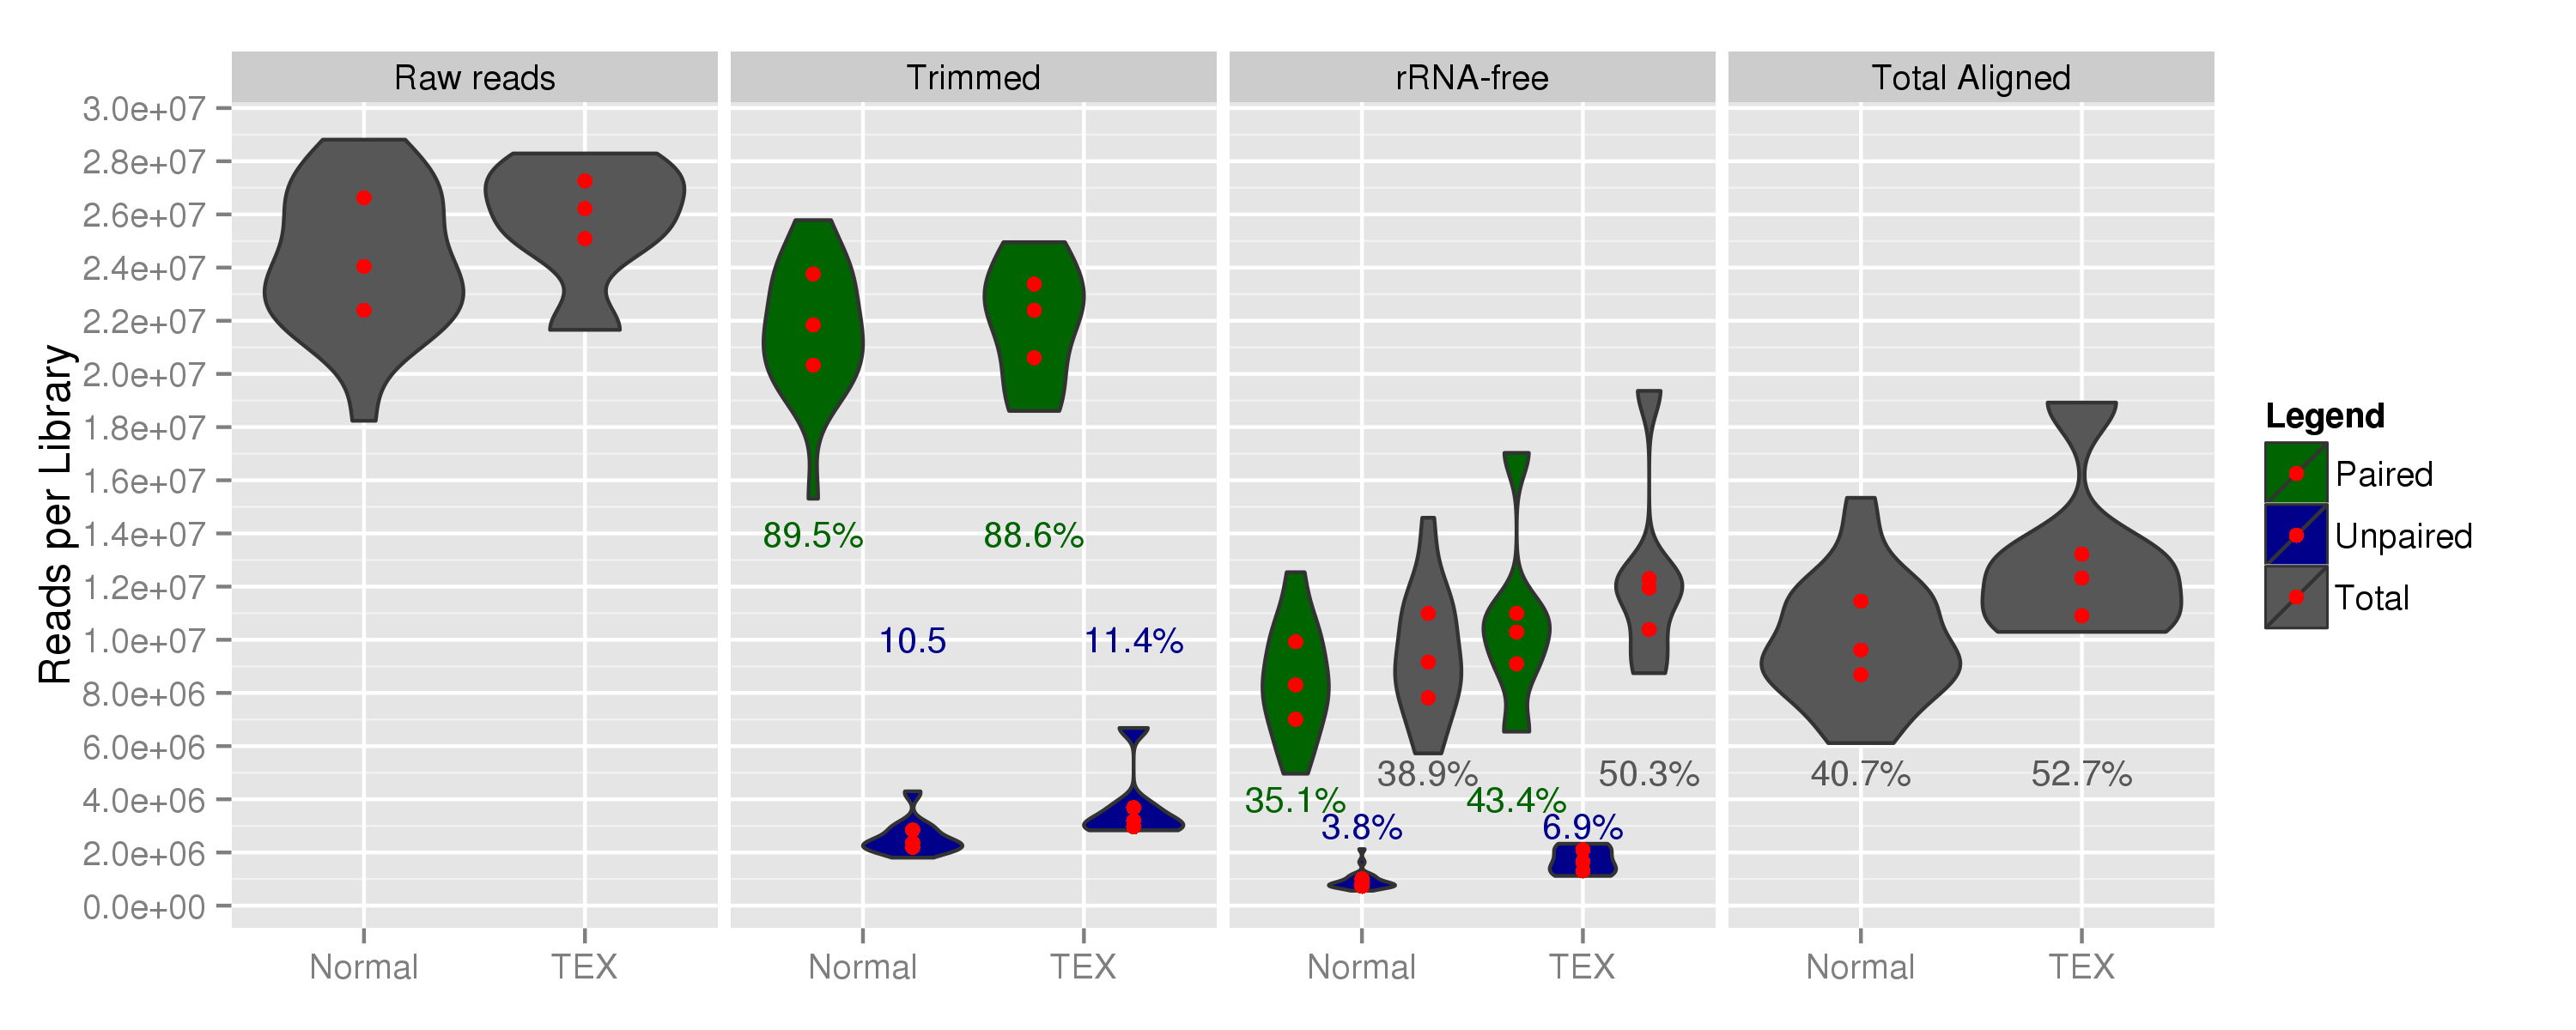
\includegraphics[width=\textheight,height=4in]{images/Sequencing/Supplemental/alignment_summary.png}
\caption{Read Trimming, Filtering, and Alignment}\label{app:alignment_summary}
Raw reads from each library were processed, resulting in both paired and unpaired reads. These reads were then aligned to rRNA sequences, with 97\% of the remaining mRNA reads aligning to the genome.
\end{minipage}}\hfill}
\end{figure}

\begin{figure}
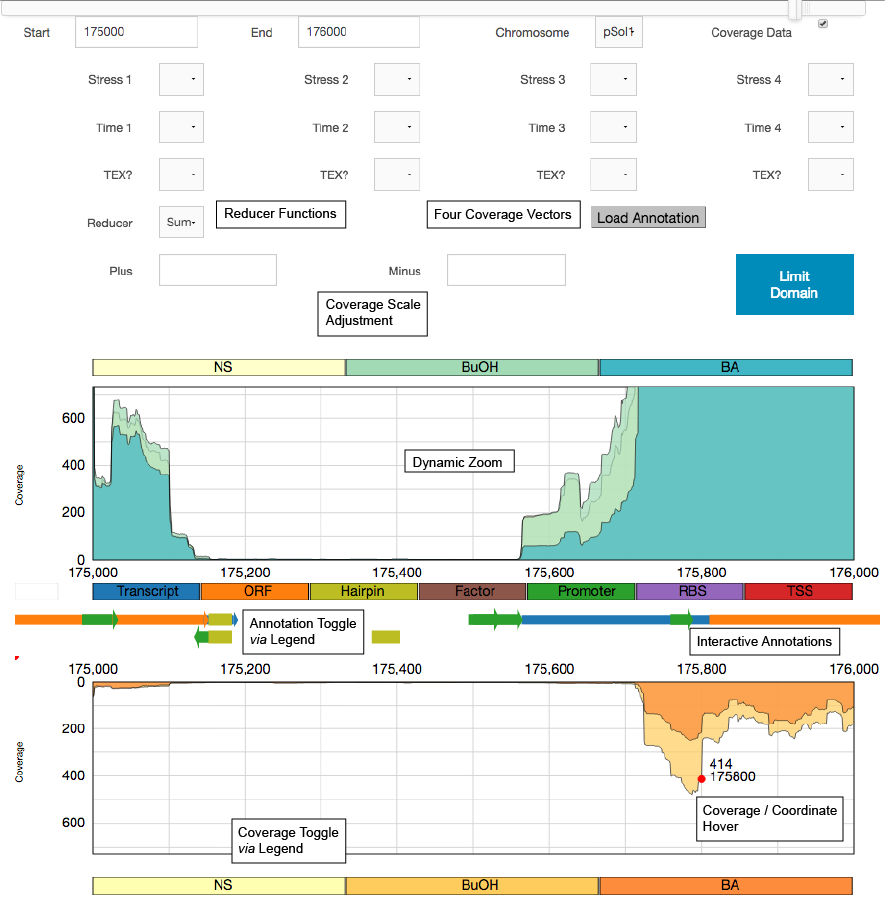
\includegraphics[width=\textwidth]{images/Assembly/Browser/Genome_browser_ui.png}
\caption{Genome Browser}\label{app:browser_ui}
The customized genome browser has unique features that facilitate the exploration of the sequencing dataset at high resolution.
\end{figure}


